\section{Experiments}
\input{Tables/combined_table}
본 장에서는 제안한 Language-Aware Skeleton Exploration Framework (\LASEF)의 효과를 다양한 실험 설정에서 체계적으로 검증한다. 실험은 스켈레톤의 구조와 생성 방식은 고정한 채, 모델 규모, 문제 난이도, 언어 자원 수준을 변화시키는 방식으로 설계되었다. 이를 통해 (1) 스켈레톤 기반 추론의 효과가 특정 조건에 국한된 현상이 아닌지, 그리고 (2) 언어 및 모델 특성에 따라 어떻게 달라지는지를 분석한다. %특히, 본 연구는 평균 성능 향상뿐 아니라 언어별 민감도와 변동성에 초점을 맞추어, 다국어 추론 환경에서 스켈레톤 활용의 가능성과 한계를 함께 논의한다.

\subsection{Experimental Setup}

\paragraph{Models based on its Scale.}
스켈레톤의 효과가 모델 규모에 따라 어떻게 달라지는지를 분석하기 위해, 본 연구에서는 기존 Structure-of-Thought를 따라~\citep{qi2025sot} 비 추론 특화 모델 중 다국어 능력이 우수하고 널리 사용되는 \textsc{Qwen2.5} 계열을 기본 모델로 선택하였다. 구체적으로, Qwen2.5-7B, 14B, 72B의 총 세 가지 서로 다른 모델 크기를 사용하여, 모델 규모가 커질수록 스켈레톤 기반 구조적 가이드의 영향이 어떻게 변화하는지를 분석한다. \textsc{Llama~3.1} 계열의 모델 또한 실험을 수행하였으며 Appendix~\ref{}에서 확인할 수 있다.

% \textsc{Llama~3.1} 계열을 기본 모델로 선택하였다. 두 모델군은 서로 다른 학습 데이터 구성과 아키텍처 특성을 가지며, 다국어 환경에서의 일반화 성능을 비교하기에 적합하다. 

\paragraph{Benchmarks based on Difficulty Levels.}
문제 난이도에 따른 스켈레톤의 영향을 확인하기 위해, 수학 추론 벤치마크를 난이도별로 구성하였다. 초급 난이도의 다국어 산술 추론을 평가하기 위해 MGSM을 사용하였고, 중간 난이도의 체계적인 수학 문제를 포함하는 MATH-500을 선택하였다. 마지막으로, 고급 난이도의 복합 추론 능력을 요구하는 PolyMath를 사용하여, 문제 구조가 복잡해질수록 스켈레톤의 효과가 어떻게 달라지는지를 분석한다.

\paragraph{Target Languages based on Resource Levels.}
언어 자원 수준에 따른 스켈레톤의 영향을 평가하기 위해, 고자원 언어부터 저자원 언어에 이르는 다양한 target 언어를 포함하였다. 고자원 언어는 대규모 사전 학습 데이터에 충분히 노출된 언어를 기준으로 선정하였으며, 저자원 언어는 학습 데이터의 상대적 희소성으로 인해 다국어 LLM에서 일관된 추론 성능을 보이기 어려운 언어들을 중심으로 구성하였다. 이를 통해 스켈레톤이 언어 자원 수준에 따라 서로 다른 역할을 수행하는지를 분석한다.

\paragraph{Evaluation Protocol.}
모든 실험은 추론 과정의 변동성을 최소화하기 위해 greedy decoding을 사용하였다. 정량적 평가는 \texttt{math-verify} 라이브러리~\citep{mathverify}를 활용하여 모델의 출력이 정답과 정확히 일치하는지를 기준으로 한 Exact Match (EM)를 측정한다. 또한 추론 능력에 대한 공정한 비교를 보장하기 위해, 출력 언어가 일관되게 유지된 경우에 한해서만 평가를 수행하였다. 구체적으로, 정답 언어가 목표 언어로 주어지는 $\ell_a=\ell_t$ 설정을 만족하는 샘플만을 평가 대상으로 포함함으로써, 언어 혼합이나 코드 스위칭으로 인한 평가 왜곡을 방지하였다. 더 구체적인 평가 방식은 Appendix~\ref{}에 기술하였다.

%\subsection{Baseline Configurations}

%제안하는 LASOF의 실험을 위해선 주어진 사용자 target 언어 $\ell_t$에 대해 질의, 스켈레톤, 추론답변 언어 즉 $(\ell_q, \ell_s, \ell_a)$를 설정해야 해야 하며 비교해야할 baseline이 필요하다. 스켈레톤은 추론 능력향상의 목적이 있기 때문에 우리는 기존 연구를 따라 두 가지 CoT기반 baseline을 수립했다. CoT기반 baseline은 CoT없는 baseline보다 일반적으로 더 높은 성능을 보이기에, 스켈레톤의 baseline으로 널리 사용된다.

%\paragraph{Target-Language CoT (\textsc{CoT-$\ell_t$}). }
%기본 설정으로, 입력 질의가 target 언어로 주어지며, 동일한 언어로 추론과 답변이 생성된다 $(\ell_t=\ell_q=\ell_a)$. 이 경우 일반적인 CoT (let's think step by step) 프롬프트를 사용하며, 스켈레톤은 적용하지 않는다.

%\paragraph{English-Pivot CoT (\textsc{CoT-$en$}).}
%입력 질의를 영어로 번역한 뒤 $(\ell_q=en)$, target 언어 $(\ell_t)$로 추론과 답변을 생성하는 설정이다. 

%[여기에 왜 질의를 영어로 번역한 baseline이 필요한가 정당성 있게 서술 필요]
% - 기존 Skeleton 연구에서 질의를 영어로 번역해 비교 실험하는 경우가 매우 많음.
% - 현실적으로, 사용자 입장에서 target 언어 $(\ell_t)$를 (e.g., 태국어)로 넣더라도 모델 자체적으로 질의를 영어로 번역해도 의미전달에 문제가 없음.

%Table~\ref{tab:combined-results}의 Method 열은 이러한 언어 구성에 따라 정리되어 있으며, 별도의 언급이 없는 한 스켈레톤 언어는 영어 $(\ell_s=\text{EN})$로 고정된다. 이후 실험 결과 분석에서는 각 언어 구성 간의 상대적인 성능 차이를 통해, 스켈레톤이 번역 효과와 구조적 가이드 효과 중 어느 요소에 의해 주로 기여하는지를 분석한다.

\subsection{Baseline Configurations}

\LASEF의 효과를 분석하기 위해서는 주어진 target 언어 $\ell_t$에 대해 질의 언어, 스켈레톤 언어, 추론 및 답변 언어로 구성된 언어 조합 $(\ell_q,\ell_s,\ell_a)$을 명시적으로 설정하고, 이에 대한 비교 기준(baseline)을 수립할 필요가 있다. 스켈레톤은 추론 성능 향상을 목적으로 하는 구조적 가이드이므로, 본 연구에서는 기존 다국어 추론 연구를 따라 Chain-of-Thought(CoT) 기반 설정을 기본 비교 기준으로 사용한다. CoT는 비구조적 프롬프트에 비해 일반적으로 더 안정적인 추론 성능을 보이므로, 스켈레톤의 기여를 평가하기 위한 적절한 기준선에 해당한다 [].

\paragraph{Target-Language CoT (\textsc{CoT-$\ell_t$}).}
입력 질의가 target 언어로 주어지며, 동일한 언어로 추론과 답변이 생성되는 설정이다 $(\ell_q=\ell_a=\ell_t)$. 일반적인 CoT 프롬프트(``Let’s think step by step, Respond in \{$\ell_t$\}'')를 사용하며, 스켈레톤은 적용하지 않는다. 이는 사용자가 자신의 모국어로 질의와 추론 과정을 모두 확인할 수 있는 가장 자연스러운 사용 시나리오에 해당한다.

\paragraph{English-Pivot CoT (\textsc{CoT-$en$}).}
입력 질의를 영어로 번역한 뒤 $(\ell_q=\text{en})$, target 언어 $\ell_t$로 추론과 답변을 생성하는 설정이다. 이 baseline은 두 가지 이유에서 필수적이다. 첫째, 기존 다국어 추론 연구들에서 영어로 번역된 질의를 기준으로 성능을 비교하는 경우가 널리 사용되어 왔으며~\citep{clp-emnlp2023,xlt-emnlp2023,trans-allneed-2025naacl}, 영어 중심으로 사전 학습된 LLM의 상한 성능을 대표하는 기준선 역할을 한다. 둘째, 실제 비영어권 사용자 환경에서도 사용자는 질의의 의미를 이미 알고 있으므로, 시스템 내부적으로 질의를 영어로 변환하더라도 의미 전달에는 큰 문제가 발생하지 않는다. 따라서 \textsc{CoT-$en$}은 번역을 통한 성능 향상이 구조적 가이드 없이도 달성 가능한 수준인지를 평가하기 위한 합리적인 비교 기준에 해당한다.

\paragraph{Skeleton baseline 언어 구성.} 
% 기존 연구들을 따라 가장 high-resource 언어인 영어로 구성했다[].
Table~\ref{tab:combined-main-table,tab:low-resource-mgsm}에서는 영어를, Figure~\ref{fig:cross-lingual-skeleton}에서는 중국어, 스페인어, 러시아어, 한국어, 태국어를 활용하였다.

\subsection{Performance across Diverse Dimensions}

%\subsubsection{Effect of English Skeleton}
Table~\ref{tab:combined-main-table}는 MGSM, MATH-500, PolyMath 세 가지 수학 추론 벤치마크에 대해, \LASEF를 영어 스켈레톤 only 환경 $(\ell_q, en, \ell_a)$ 에서의 성능을 비교한 결과이다.

\paragraph{Overall.}
실험 결과, 영어 스켈레톤의 도입은 모델의 크기, 벤치마크의 난이도, 그리고 언어의 자원 수준에 따라 상이한 효과를 보였다. 구체적으로 1) 모델 크기가 작을수록, 2) 문제의 난이도가 낮을수록, 3) 저자원 언어일수록 성능 향상의 폭이 두드러졌다. 예를 들어, Qwen2.5-7B-Instruct 모델은 MGSM 벤치마크의 스와힐리어(sw) \textsc{CoT-$en^{\dagger}$} 설정에서 63.1점에서 71.7점으로 +8.6점 향상되었으나, 더 큰 모델인 Qwen2.5-72B-Instruct에서는 오히려 85.5점에서 86.7점으로 소폭 상승(+1.2점)하거나 Qwen2.5-14B-Instruct에서는 정체되는 경향 보였다. 이는 스켈레톤 방식이 모든 상황에서 일관된 이득을 보장하기보다는 특정 조건하에서 유의미한 variation을 가짐을 시사한다.
한편, 질의를 영어로 번역하여 추론하는 \textsc{CoT-$en^{\dagger}$} 설정은 타겟 언어로 직접 추론하는 \textsc{CoT-$\ell_t$} 대비 월등한 성능을 보이며, 대규모 데이터로 학습된 언어 모델의 강력한 영어 우선순위(English prior)를 재확인시켜 준다. 실제로 Qwen2.5-7B 모델을 이용한 MGSM 벤치마크 실험에서, \textsc{CoT-$en^{\dagger}$}는 \textsc{CoT-$\ell_t$}의 65.3점을 크게 상회하는 평균 76.5점을 기록하였다. 이는 단순한 언어 변환만으로도 상당한 성능 향상을 이끌어낼 수 있음을 시사하는 동시에, 본 연구에서 분석하는 스켈레톤 방법론의 효용성을 검증하기 위해 반드시 고려해야 할 강력한 비교 기준이 된다.
% 한편, 질의를 영어로 번역하여 추론하는 \textsc{CoT-$en^{\dagger}$} 설정은 대부분의 경우 \textsc{CoT-$\ell_t$} 대비 월등히 높은 성능(예: Qwen2.5-7B MGSM 평균 76.5점 vs. 65.3점)을 기록하며, 영어 데이터로 대규모 학습된 언어 모델의 강력한 영어 우선순위(English prior)를 재확인시켜 주었다. 이는 단순 질의 번역만으로도 상당한 성능 개선이 가능함을 보여주는 동시에, 스켈레톤 방법론의 효과를 검증하기 위한 중요한 비교 기준이 된다.

\paragraph{Bridging the Resource Gap}
% \paragraph{Do Gains Depend on Language Resources?}
language resource 수준에 따른 차이는 매우 뚜렷하게 나타난다. 영어 스켈레톤은 중국어(zh), 스페인어(es)와 같은 고자원 언어보다, 스와힐리어(sw)와 같은 저자원 언어에서 훨씬 큰 효과를 보인다. Qwen2.5-7B-Instruct의 경우, CoT-$en^{\dagger}$ 설정에서 MGSM의 스와힐리어 성능은 63.1에서 영어 스켈레톤 적용시 71.7로 +8.6 향상된다. 반면, 동일한 설정에서 중국어와 스페인어는 각각 +0.0, +1.6에 그친다. 이러한 경향은 다른 모델 규모와 벤치마크에서도 일관되게 관찰된다. 예를 들어 Qwen2.5-72B-Instruct의 CoT-$en^{\dagger}$ 설정에서 MATH-500 평균 성능은 61.5에서 62.4로 +0.9 증가하는데, 이 중 가장 큰 향상은 역시 스와힐리어(+3.7)에서 나타난다. 이러한 결과들은 low resource 자체만으로는 복잡한 추론 과정을 전개하기 어려울 때, 상대적으로 추론 능력이 강력한 영어로 스켈레톤을 생성하는 것이 보다 안정적으로 유지하도록 돕는 역할을 한 것으로 보인다.

% 상대적으로 추론 능력이 강력한 영어로 스켈레톤을 생성하는 것이 논리적 완결성을 보완해 줌을 의미한다.

\paragraph{Does Scaling Always Guarantee Improvement?}
모델 규모의 측면에서는 작은 모델일 수록 영어 스켈레톤으로 얻는 이득이 컸으며, 모델 규모가 커질 수록 그 효과가 감소하거나 역효과가 발생하는 경향이 관찰되었다. Qwen2.5-7B, 14B 규모의 모델은 전반적인 벤치마크 모두에서 스켈레톤 적용 후 성능 향상을 보였으나(+0.9--2.5) Qwen2.5-72B-Instruct는 MGSM에서 CoT-$\ell_t$에서, PolyMath CoT-$en$에서 스켈레톤 적용 후 평균 0.2의 성능 하락을 기록하였다. 이는 대규모 모델에서는 외부에서 강제된 영어 스켈레톤이 불필요한 제약으로 작용할 수 있음을 시사한다.

% \paragraph{Difficulty of Benchmarks}
\paragraph{Does Benchmark Difficulty Limit the Gains?}
벤치마크 난이도에 따른 성능 변화를 살펴보면, 난이도가 낮은 벤치마크일수록 스켈레톤의 기여도가 높았다. Qwen2.5-7B-Instruct 모델을 기준으로 가장 난이도가 낮은 MGSM에서는 +2.2의 성능 향상을 보인 반면, 난이도가 중간인 MATH-500에서는 +1.8, 가장 어려운 PolyMath에서는 +1.2로 성능 향상 폭이 점차 줄어들었다. 이는 고난이도 문제일수록 단순한 스켈레톤 생성뿐만 아니라, 고난도의 연산 추론 과정이 요구되기 때문에 스켈레톤만으로는 해결하기 어려운 한계가 존재함을 보여준다.

% \subsection{Skeleton in Low-Resource Languages}
\subsection{Robustness of English Skeletons in Low-Resource Languages}
\begin{table}[!t]
\centering
\resizebox{\columnwidth}{!}{
\begin{tabular}{lrrrr}
\toprule
\multirow{2}{*}{\textbf{Language}} &
\multicolumn{2}{c}{\textbf{$\ell_t,en,\ell_t$}} &
\multicolumn{2}{c}{\textbf{$en^{\dagger},en,\ell_t$}}\\
\cmidrule(lr){2-3}\cmidrule(lr){4-5}
 & \textsc{CoT-$l_t$} & +\textsc{Skeleton} & \textsc{CoT-$en^{\dagger}$} & +\textsc{Skeleton} \\
\midrule
\rowcolor{gray!10}\multicolumn{5}{c}{\textbf{\textit{Qwen2.5-7B-Instruct}}}\\
\midrule
kk & 40.08 & 51.42 (\textcolor{red}{+11.34}) & 62.82 & 72.22 (\textcolor{red}{+9.40}) \\
ky & 33.33 & 37.86 (\textcolor{red}{+4.53}) & 61.92 & 65.69 (\textcolor{red}{+3.77}) \\
mn & 27.16 & 33.33 (\textcolor{red}{+6.17}) & 66.96 & 64.78 (\textcolor{blue}{-2.18}) \\
ug & 27.13 & 37.65 (\textcolor{red}{+10.52}) & 57.14 & 60.37 (\textcolor{red}{+3.23}) \\
hy & 50.81 & 56.05 (\textcolor{red}{+5.24}) & 64.49 & 73.88 (\textcolor{red}{+9.39}) \\
lo & 25.51 & 23.48 (\textcolor{blue}{-2.03}) & 48.54 & 48.95 (\textcolor{red}{+0.41}) \\
eu & 20.76 & 19.92 (\textcolor{blue}{-0.84}) & 65.62 & 74.55 (\textcolor{red}{+8.93}) \\
mt & 25.65 & 20.00 (\textcolor{blue}{-5.65}) & 62.11 & 58.59 (\textcolor{blue}{-3.52}) \\
am & 8.23  & 10.29 (\textcolor{red}{+2.06})  & 39.63 & 32.93 (\textcolor{blue}{-6.70}) \\
ne & 54.29 & 52.65 (\textcolor{blue}{-1.64}) & 74.58 & 78.81 (\textcolor{red}{+4.23}) \\
si & 10.16 & 12.20 (\textcolor{red}{+2.04})  & 37.14 & 35.92 (\textcolor{blue}{-1.22}) \\
ps & 26.46 & 26.91 (\textcolor{red}{+0.45}) & 37.62 & 47.03 (\textcolor{red}{+9.41}) \\
sd & 20.27 & 22.07 (\textcolor{red}{+1.80}) & 64.81 & 68.52 (\textcolor{red}{+3.71}) \\
pa & 51.41 & 52.21 (\textcolor{red}{+0.80}) & 55.87 & 52.63 (\textcolor{blue}{-3.24}) \\
gu & 44.35 & 47.98 (\textcolor{red}{+3.63}) & 59.84 & 60.64 (\textcolor{red}{+0.80}) \\
mr & 45.34 & 46.96 (\textcolor{red}{+1.62}) & 75.41 & 74.18 (\textcolor{blue}{-1.23}) \\
or & 44.35 & 43.95 (\textcolor{blue}{-0.40}) & 36.84 & 38.06 (\textcolor{red}{+1.22}) \\
ta & 47.79 & 49.80 (\textcolor{red}{+2.01}) & 69.48 & 69.08 (\textcolor{blue}{-0.40}) \\
ml & 42.74 & 46.37 (\textcolor{red}{+3.63}) & 62.25 & 64.66 (\textcolor{red}{+2.41}) \\
\midrule
\textbf{AVG.}
 & 33.99 & 36.37 (\textcolor{red}{+2.38})
 & 58.06 & 60.08 (\textcolor{red}{+2.02}) \\
\bottomrule
\end{tabular}
}
\caption{\small Performance comparison on 19 low-resource languages (MGSM) using \textsc{Qwen2.5-7B} with English Skeleton. CoT-$en^{\dagger}$: English-translated queries via Google Translate. Parentheses show $\Delta$ gains.}
\label{tab:low-resource-mgsm}
    \vspace{-0.15in}
\end{table}

앞선 분석을 통해 영어 스켈레톤의 이점이 소규모 모델, 낮은 난이도의 벤치마크, 그리고 저자원 언어 조건에서 가장 두드러짐을 확인하였다. 본 절에서는 이를 보다 심층적으로 검증하기 위해, Qwen2.5-7B-Instruct 모델을 사용하여 MGSM 벤치마크 내 19개 저자원 언어에 대한 성능을 분석한다. 분석 대상에는 학습 데이터 비중이 극히 낮은 위구르어(ug), 키르기스어(ky), 카자흐어(kk) 등이 포함되며, 이러한 환경에서 Skeleton 기반 CoT가 일관된 성능 개선을 제공하는지 면밀히 살펴본다. Appendix~\ref{}에서 저자원 언어를 선택한 기준을 설명한다.

Table~\ref{tab:low-resource-mgsm}은 원본 언어 입력($\ell_t$)과 영어 번역 입력($en^{\dagger}$) 설정 각각에 대한 성능 변화를 요약한다. 실험 결과, 영어 스켈레톤은 저자원 언어 환경 전반에서 견고한 성능 향상을 이끌어냈다. 구체적으로 스켈레톤 적용 시 원본 질의 설정에서는 평균 +2.38, 영어 번역 질의 설정에서는 평균 +2.02의 성능 개선이 관찰되었다.

첫째, Native Input ($CoT-\ell_t$) 설정의 경우, 카자흐어(kk, +11.34)와 위구르어(ug, +10.52) 등 일부 언어에서는 스켈레톤이 모델의 잠재된 추론 능력을 대폭 이끌어내는 결과를 보였다. 그러나 몰타어(mt, -5.65)와 같이 오히려 성능이 하락하는 사례도 존재하여, 언어별 효과의 편차(high variance)가 큼을 확인하였다.

둘째, Translated Input ($CoT-en$) 설정에서는 영어 스켈레톤의 효과가 더욱 안정적으로 나타났다.우선, 단순 질의 번역만으로도 평균 점수가 33.99점에서 58.06점으로 비약적으로 상승하여, 저자원 언어 환경에서 질문을 영어로 번역하여 제공하는 것이 효과적임을 의미한다. 이에 추가적으로 영어 스켈레톤을 결합할 경우 +2.02점의 추가적인 성능 향상이 뒤따랐다. 특히 아르메니아어(hy, +9.39), 바스크어(eu, +8.93), 파슈토어(ps, +9.41) 등에서는 번역된 질문 위에 논리적 구조(Skeleton)가 더해지며 큰 폭의 성능 향상을 기록하였다. 

종합하면, 저자원 언어 환경에서는 언어적 장벽을 완화하는 `질의 번역'과 추론 과정을 구조화하는 `영어 스켈레톤'을 결합할 때 모델의 잠재력이 가장 효과적으로 발현된다. 이는 Skeleton 기반 CoT가 극저자원 언어 환경에서도 유효한 추론 보조 수단이 될 수 있음을 시사한다.

\subsection{Is English the Only Solution for Low-Resource Languages?}
\label{sec:low-resource-nonen}
% \begin{figure}[!ht]
%     \centering
%     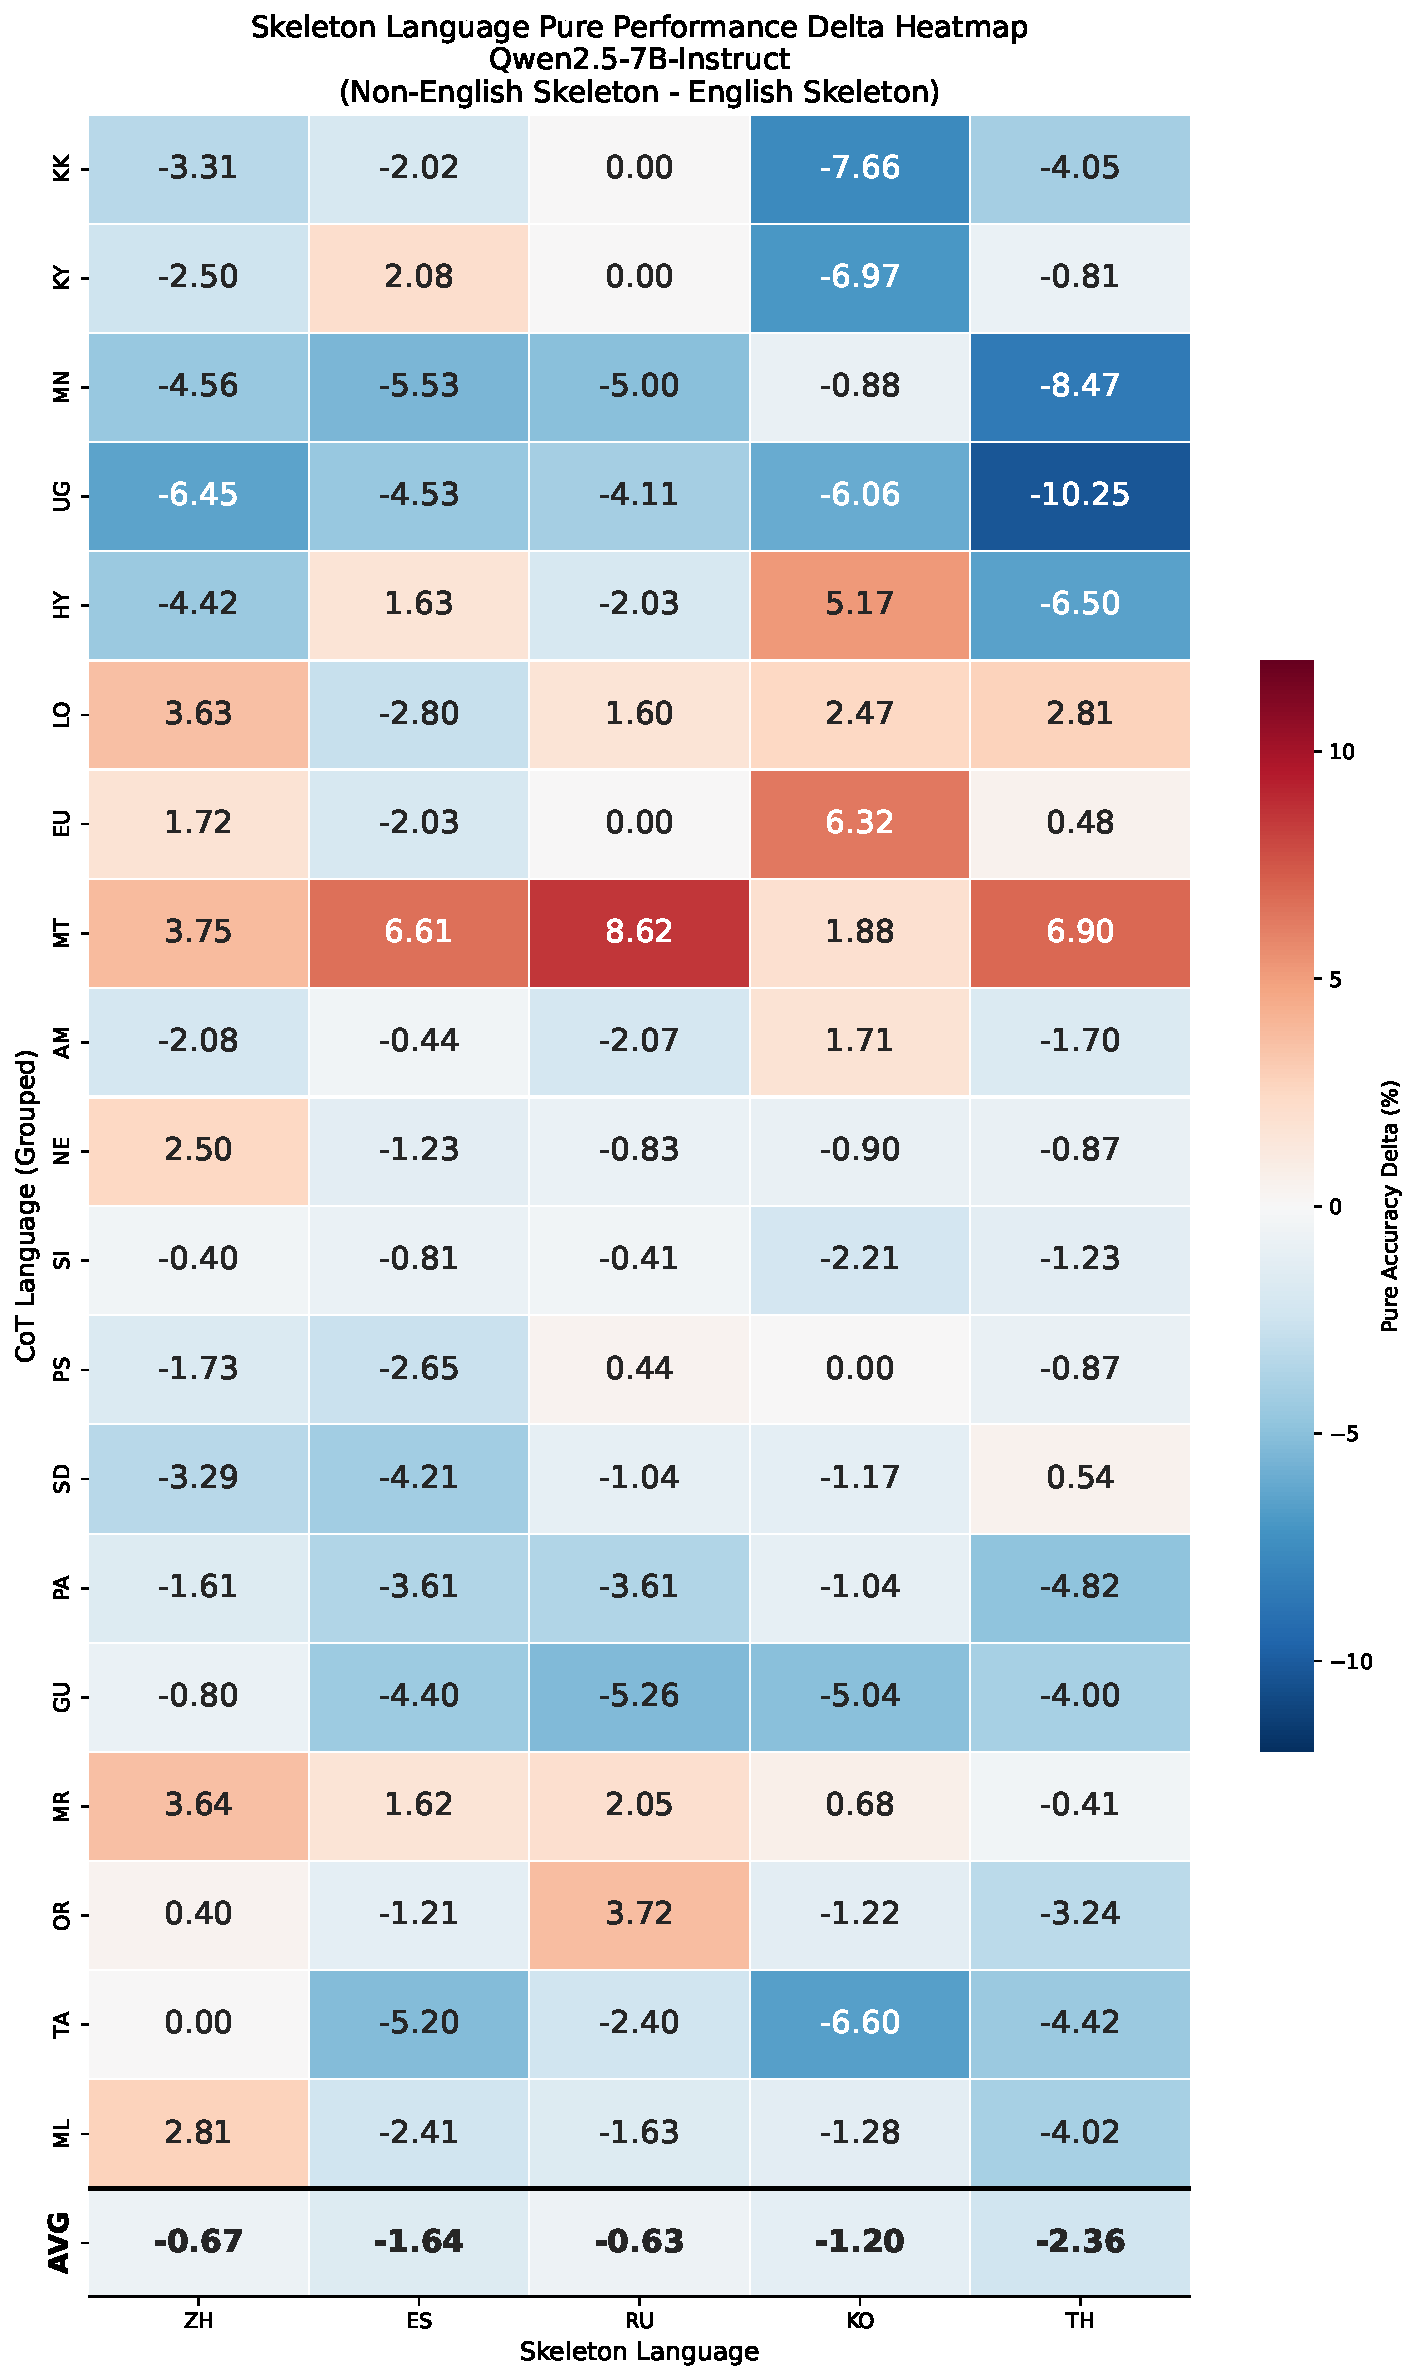
\includegraphics[width=\linewidth]{Figures/Images/Qwen2.5-7B-Instruct_single_pure_delta_heatmap_sorted.pdf}
%     \caption{\small Performance differences (Non-English $-$ English) on the MGSM under the CoT-$\ell_t$ setting with \textsc{Qwen2.5-7B}. English skeleton is replaced with five Non-English skeletons (ZH, ES, RU, KO, and TH). While English generally provides a stable default skeleton language, several target languages exhibit gains with specific Non-English skeletons, indicating that skeleton effectiveness is language-dependent.}
%     \label{fig:cross-lingual-skeleton}
%     \vspace{-0.15in}
% \end{figure}

\begin{figure*}[!ht]
    \centering
    \captionsetup[subfigure]{labelformat=simple, labelsep=space}
    \renewcommand\thesubfigure{(\alph{subfigure})}
    \begin{subfigure}[t]{0.48\linewidth}
        \centering
        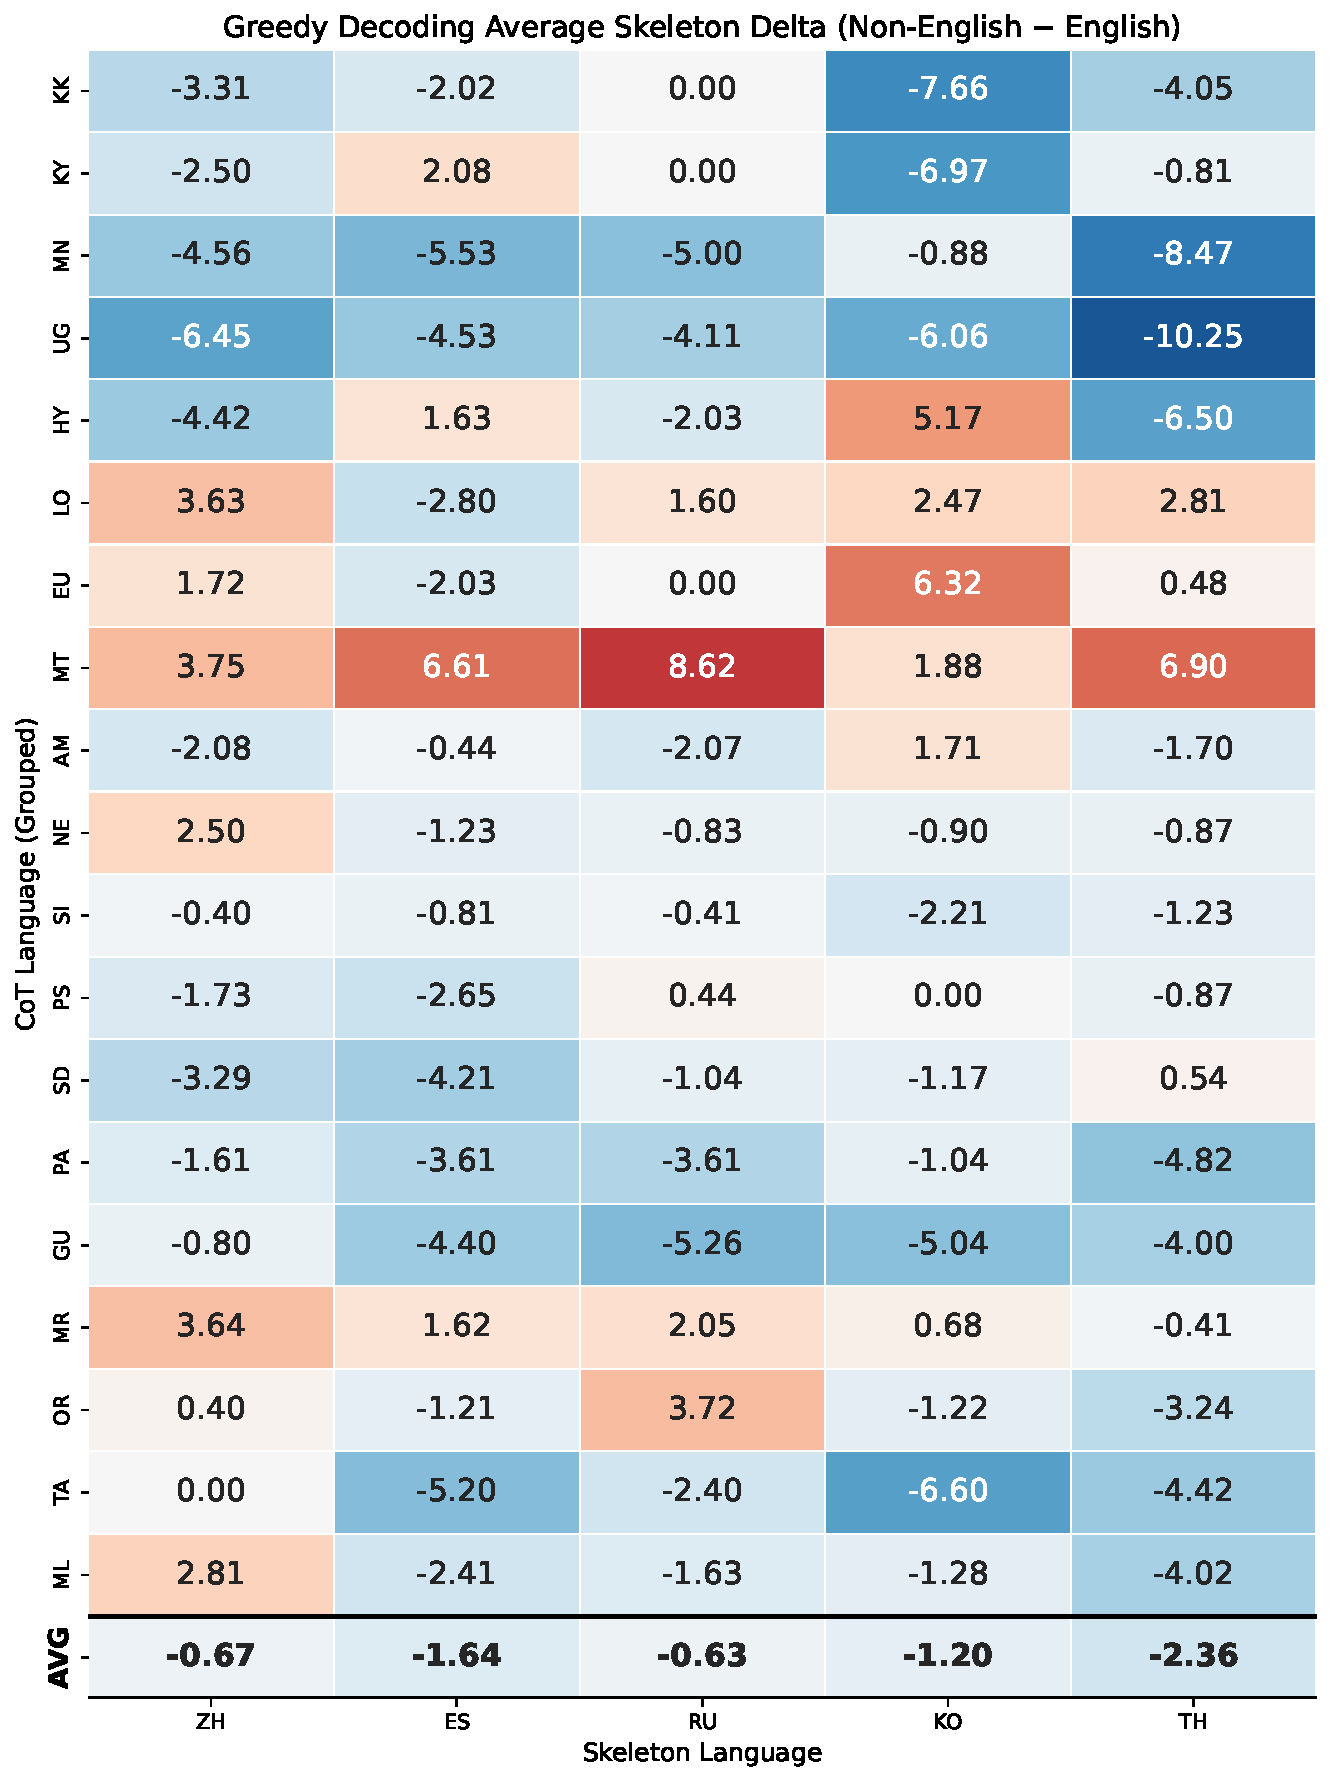
\includegraphics[width=\linewidth]{Figures/Images/greedy.pdf}
        \caption{Greedy Decoding (single rollout)}
        \label{fig:heatmap-greedy}
    \end{subfigure}
    \hfill
    \begin{subfigure}[t]{0.48\linewidth}
        \centering
        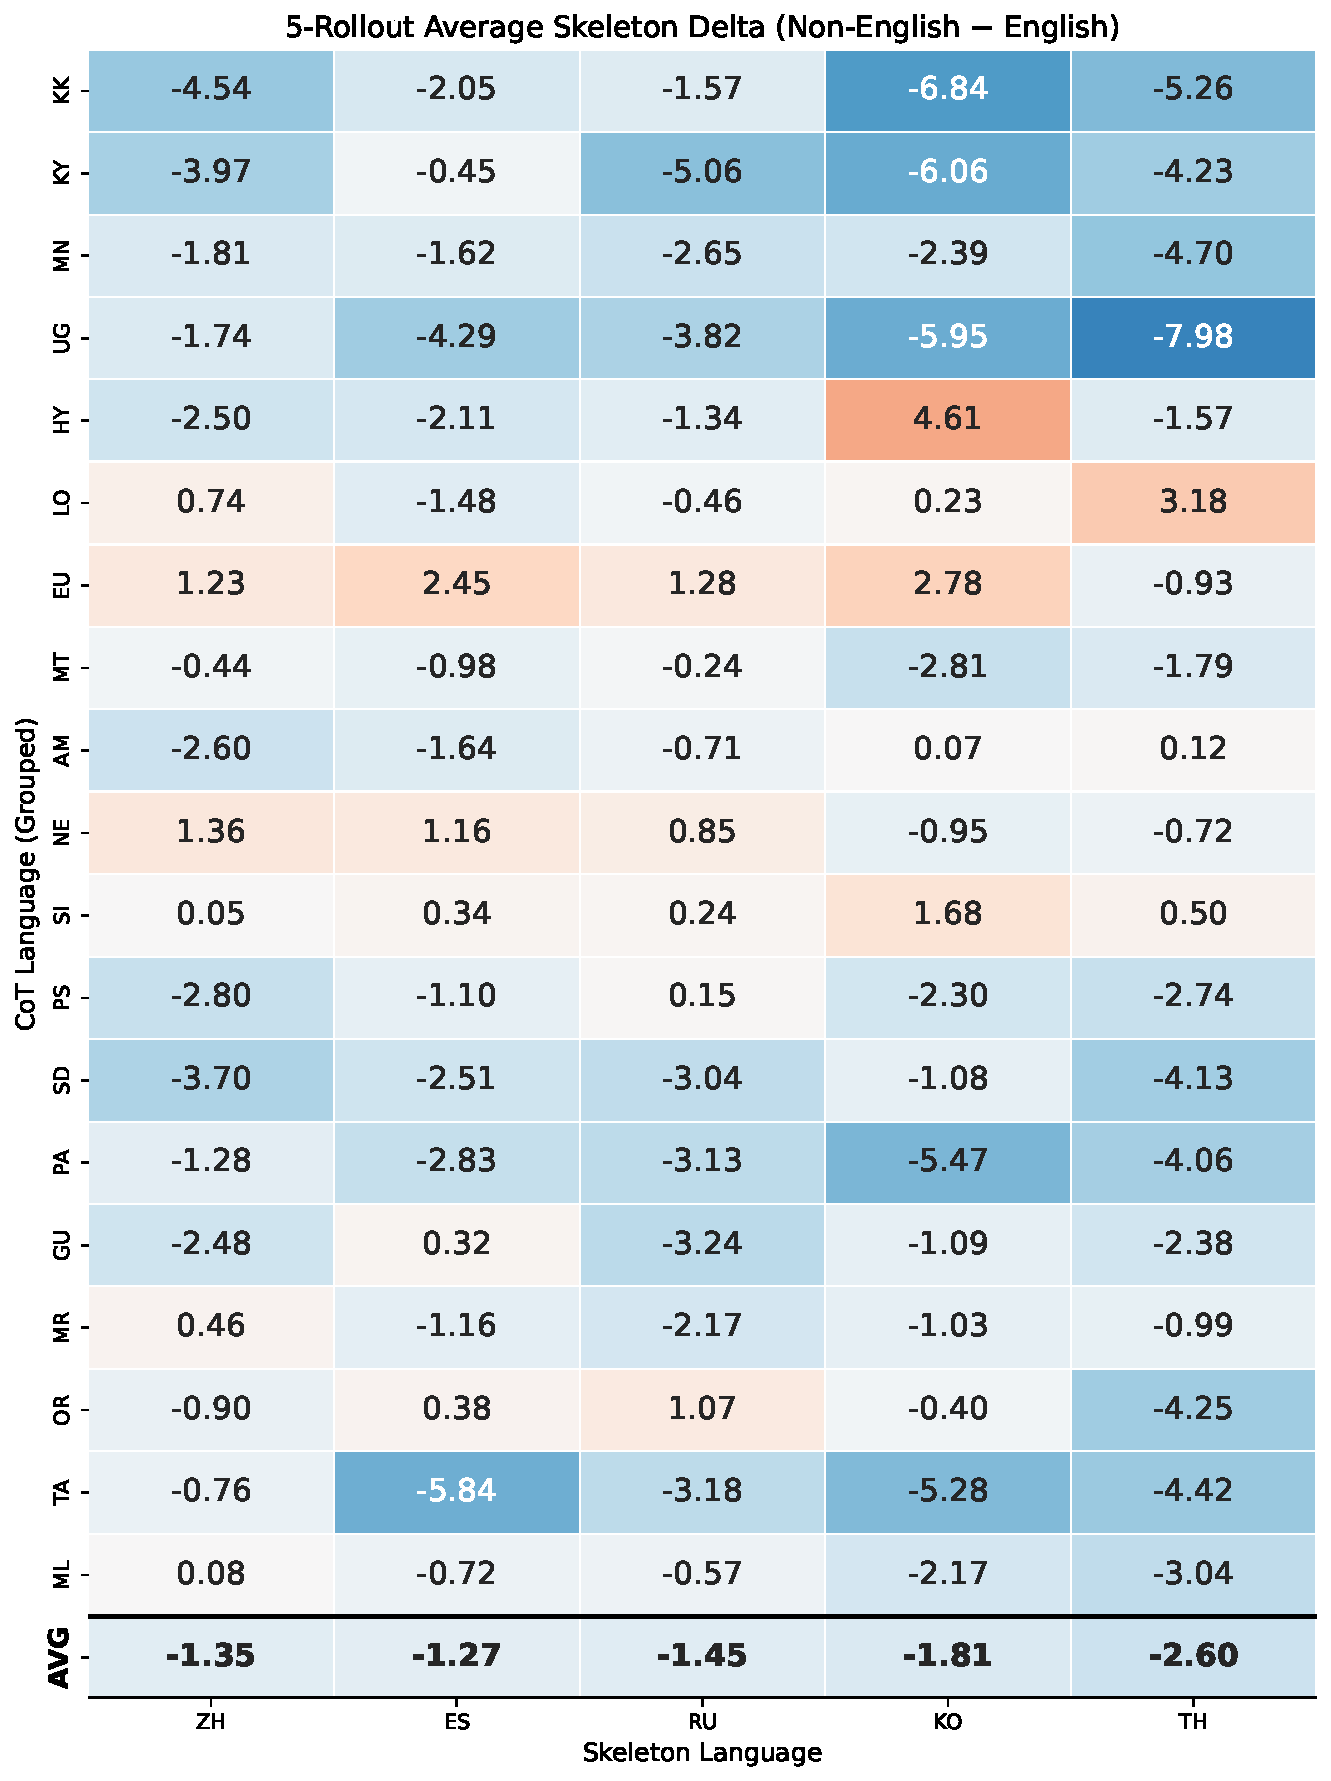
\includegraphics[width=\linewidth]{Figures/Images/5rollout.pdf}
        \caption{Multi-rollout ($T{=}0.7$, $N{=}5$)}
        \label{fig:heatmap-rollout5}
    \end{subfigure}
    \caption{\small Performance differences (Non-English $-$ English) on MGSM under CoT-$\ell_t$ with \textsc{Qwen2.5-7B}. The English skeleton is replaced with five Non-English skeletons (ZH, ES, RU, KO, TH); the same skeleton set is used in both panels. \textbf{(a)} Greedy decoding (single rollout). \textbf{(b)} Multi-rollout sampling ($T{=}0.7$, $N{=}5$).}
    \label{fig:cross-lingual-skeleton}
    \vspace{-0.15in}
\end{figure*}
앞선 섹션에서 우리는 영어 스켈레톤이 전반적으로 효과적인 추론 보조 도구임을 확인하였다. 그러나 Table~\ref{tab:low-resource-mgsm}의 \textsc{CoT-$\ell_t$} 결과를 자세히 살펴보면, 영어가 모든 저자원 언어에 대해 만능 해결책은 아님을 알 수 있다. 19개 저자원 언어 중 5개 언어(lo, eu, mt, ne, or)에서 영어 스켈레톤 적용 시 오히려 성능이 하락하는 현상(\textcolor{blue}{$-$})이 관찰되었다. 본 절에서는 제안하는 \LASEF를 더욱 다양한 언어에 적용함으로써, 스켈레톤 언어 선택이 고정된 규칙으로 결정될 수 없음을 보이고, 타겟 언어의 특성에 따라 그 효과가 달라질 수 있음을 체계적으로 분석한다.
% 스켈레톤 언어 조합을 찾는 과정을 심층적으로 분석한다.
%
% 앞선 섹션에서 우리는 영어 스켈레톤이 저자원 언어 환경에서 효과적인 추론 보조 도구임을 확인하였다. 본 절에서는 제안하는 \LASEF를 더욱 다양한 언어에 적용해 최적의 스켈레톤 언어조합을 찾는 과정을 심층적으로 분석한다.

\paragraph{General Trends: English as a Stable Anchor.}
Figure~\ref{fig:cross-lingual-skeleton}는 CoT-$\ell_t$ 환경에서, Qwen2.5-7B-Instruct 모델을 사용하여 영어 스켈레톤을 5가지 비영어(Non-English) 스켈레톤(중국어, 스페인어, 러시아어, 한국어, 태국어)으로 대체했을 때의 성능 차이(Non-English $-$ English)를 나타낸다. 전반적인 경향성을 볼 때, 영어를 제외한 다른 언어 스켈레톤을 일괄적으로 적용하면 언어별 평균 성능이 0.56점에서 2.32점까지 감소하였다. 이러한 결과는 영어가 대부분의 언어에 대해 가장 보편적이고 안정적인 추론 스켈레톤(anchor)으로 기능함을 재확인시켜준다. 그러나 개별 언어, 특히 영어 스켈레톤이 부정적 효과를 보였던 언어들을 분석하면 주목할 만한 예외가 관찰된다.
% 전반적으로 모든 비영어 스켈레톤 설정에서 언어별 평균 성능은 0.56에서 2.32점까지 감소하였다. 이러한 결과는 영어가 대부분의 언어에 대해 가장 보편적이고 안정적인 추론 스켈레톤(anchor)으로 기능함을 재확인시켜준다. 그러나 언어별 세부 결과를 살펴보면, 언어적 유사성(linguistic affinity)이나 공통된 문화적 배경을 공유하는 특정 언어 쌍에서는 비영어 스켈레톤이 영어보다 우수한 성능을 보이는 주목할 만한 예외가 관찰된다. 

\paragraph{Linguistic Affinity and Unexpected Gains.}
Table~\ref{tab:low-resource-mgsm}에서 영어 스켈레톤 적용 시 성능 감소를 겪었던 언어들은, 언어적 뿌리나 문법 구조를 공유하는 특정 언어 스켈레톤을 만났을 때 주목할만한 성능 향상을 기록하였다.
% 언어적 뿌리나 문화적 배경을 공유하는 특정 언어 쌍에서는 비영어 스켈레톤이 영어보다 우수한 성능을 보이는 경우가 존재하였다.

대표적으로 \textsc{Lao (lo)}의 경우, 영어 스켈레톤을 적용했을 때 성능이 하락하였으나($-2.03$), 영어 대신 \textsc{Thai (th)} 스켈레톤을 사용했을 때 성능이 2.81 포인트 향상되었다. 우리는 이것이 Tai--Kadai 어족 내의 높은 문법·어휘적 유사성이 번역 과정의 정보 손실을 최소화하고 직접적인 지식 전이를 촉진했을 것이라 추측한다. 

유사하게, 고립어인 \textsc{Basque (eu)} 또한 영어 스켈레톤에서는 성능이 소폭 하락($-0.84$)하였으나, 같은 교착어이자 SOV 어순을 공유하는 \textsc{Korean (ko)} 스켈레톤을 사용했을 때 영어대비 +6.32점의 이득을 얻었다. 이러한 관찰 결과는 구조적 정렬이 추론 과정의 정합성에 긍정적으로 작용했을 가능성을 시사한다.

% 대표적으로 \textsc{Lao (lo)}의 경우, 영어 대신 \textsc{Thai (th)} 스켈레톤을 사용했을 때 성능이 2.81 포인트 향상되었다. 우리는 이것이 Tai--Kadai 어족 내의 높은 문법·어휘적 유사성이 번역 과정의 정보 손실을 최소화하고 직접적인 지식 전이를 촉진했을 것이라 추측한다. 유사하게 \textsc{Kazakh (kk)}와 \textsc{Kyrgyz (ky)}에서도 \textsc{Russian (ru)} 스켈레톤이 영어와 대등하거나(+0.00), 소폭 우세한(+0.47) 성능을 기록하였다.

% 또한, 고립어인 \textsc{Basque (eu)}는 같은 교착어이자 SOV 어순을 공유하는 \textsc{Korean (ko)} 스켈레톤을 사용했을 때 영어대비 +6.32점의 이득을 얻었다. 이러한 관찰 결과는 구조적 정렬이 추론 과정의 정합성에 긍정적으로 작용했을 가능성을 시사한다.

주목할 점은 \textsc{Maltese (mt)}의 사례이다. 영어 스켈레톤을 적용 시 가장 큰 폭의 성능 하락($-5.65$)을 겪었으나, 로망스어군의 영향을 받은 몰타어는 \textsc{Spanish (es)} 스켈레톤에서 +6.60점의 향상을 보였다. 또한, 흥미롭게도 언어학적 거리가 먼 \textsc{Russian (ru)} 스켈레톤에서 이보다 더 높은 +9.05점의 성능 향상을 기록하였다. 이는 스켈레톤의 전이 효과가 단순한 언어적 유사성만으로는 완전히 설명되지 않는 복합적인 요인에 기인할 수 있음을 보여준다.

\paragraph{Linguistic Affinity is Not Enough.}
반면, 지리적 인접성이나 문자 체계의 공유가 반드시 긍정적 전이를 보장하지는 않는다는 결과 또한 관찰된다. \textsc{Mongolian (mn)}은 키릴 문자를 공유함에도 러시아어 스켈레톤에서 $-5.53$의 성능 하락을 보였다. 이는 \textsc{Kazakh (kk)}와 \textsc{Kyrgyz (ky)}의 러시아 스켈레톤의 긍정적 영향과는 정반대의 경향을 보인다. 또한, \textsc{Uyghur (ug)}는 지리적으로 인접한 중국어 스켈레톤에서 $-6.45$의 하락을 기록하였다. 이러한 대조적인 결과는 표면적인 유사성만으로는 부족하며, 사전학습 데이터 내에서 두 언어가 실제 문맥 안에서 얼마나 자주 함께 등장했는지에 대한 co-occurrence frequency와 데이터의 절대적인 양 등 잠재적인 요인이 함께 고려되어야하는 것으로 보인다.


\paragraph{The Necessity of LASEF.}
결론적으로, 영어가 가장 강력한 general solution임은 분명하지만, Table~\ref{tab:low-resource-mgsm}와 Figure~\ref{fig:cross-lingual-skeleton}의 결과는 영어가 유일한 해답은 아님을 시사한다. 특히 영어 스켈레톤이 효과를 발휘하지 못하는 환경에서, 타겟 언어와 높은 호환성을 보이거나 구조적으로 잘 정렬된 대체 언어 스켈레톤은 성능 회복의 열쇠가 될 수 있다. 이는 스켈레톤 언어의 선택이 고정된 규칙이 아니라, 타겟 언어의 특성과 모델의 데이터 분포에 맞춰 유동적으로 최적화되어야 할 핵심적인 설계 변수임을 의미한다. 따라서, 이러한 최적의 조합을 체계적으로 탐색하는 \LASEF 의 필요성은 더욱 강조된다.

% 그러나 동시에, 타겟 언어와 언어학적·통계적 연관성이 높은 중·고자원 언어를 활용할 경우 영어보다 더 효율적인 추론이 가능함을 입증한다. 특히 앞서 관찰된 불규칙한 전이 효과(e.g., Basque, Mongolian)는 단순한 언어학적 유사성만으로는 최적의 스켈레톤 언어를 예단하기 어려움을 시사한다. 이는 스켈레톤 언어 선택이 고정된 규칙이 아닌 타겟 언어의 특성과 데이터 분포에 따라 유동적으로 최적화되어야 하는 중요한 설계 변수임을 의미하며, 이를 체계적으로 탐색하는 \LASEF 의 필요성을 강력하게 지지한다.
% 결론적으로, Figure~\ref{fig:cross-lingual-skeleton}의 결과는 영어가 여전히 가장 안정적인 anchor임을 재확인시켜 준다. 그러나 동시에, 타겟 언어와 언어학적·통계적 연관성이 높은 중·고자원 언어를 활용할 경우 영어보다 더 효율적인 추론이 가능함을 입증한다. 특히 앞서 관찰된 불규칙한 전이 효과(e.g., Basque, Mongolian)는 단순한 언어학적 유사성만으로는 최적의 스켈레톤 언어를 예단하기 어려움을 시사한다. 이는 스켈레톤 언어 선택이 고정된 규칙이 아닌 타겟 언어의 특성과 데이터 분포에 따라 유동적으로 최적화되어야 하는 중요한 설계 변수임을 의미하며, 이를 체계적으로 탐색하는 \LASEF 의 필요성을 강력하게 지지한다.
% 결론적으로, Figure~\ref{fig:cross-lingual-skeleton}의 결과를 토대로 첫번째, 영어 스켈레톤이 여전히 안정적인 anchor로서 수행함을 재확인했다. 두번째로, 타겟 언어와 언어학적·통계적 거리가 가까운 중,고자원 언어를 여러 후보로 \LASEF를 통해 확인 후 스켈레톤으로 채택하는 것이 더 효율적일 수 있음을 입증한다. 이는 스켈레톤 기반 추론에서 언어 선택이 고정된 규칙이 아니라, 타겟 언어의 특성과 데이터 분포에 따라 최적화될 수 있는 중요한 설계 변수임을 의미한다.